
\documentclass{standalone}

%\documentclass[convert]{standalone}
% convert: in addition to pdf output files, png files are created
% convert options does work properly with -output-directory option of latexmk

\usepackage{tikz-feynman}
\tikzfeynmanset{compat=1.1.0}


\begin{document}
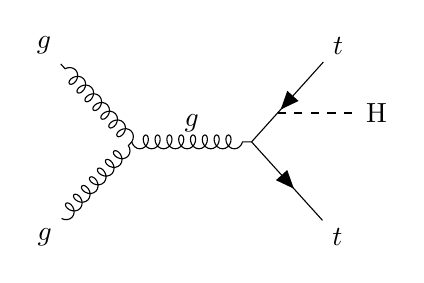
\begin{tikzpicture}
          \begin{feynman}
            \diagram [horizontal=a to b] {
            % draw s-channel gg->ttbar as usual
              i1 [particle=\(g\)]
                -- [gluon] a
                -- [gluon] i2 [particle=\(g\)],
              a -- [gluon, edge label=\(g\)] b,
              f1 [particle=\(t\)]
                -- [fermion] b
                -- [fermion] f2 [particle=\(t\)]],
            };

            % add vertex for FSR at 0.3 between vertex (b) and (f1)
            % add end vertex for FSR (with label H), then draw line between FSR vertices
            \vertex at ($(b)!0.3!(f1)$) (fsr_start);
            \vertex [right=1cm of fsr_start] (fsr_end) {H};
            \draw [scalar] (fsr_start) -- (fsr_end);
          \end{feynman}
        \end{tikzpicture}
\end{document}
